
%%%% OK

In this section, we present our own large-scale emulation platform called AndroFleet that provides us a good testing tool for our approach and the evaluation protocol that we will conduct.

Applications developed for the mobile platforms are difficult to test.
When comes the time of the evaluation, 3 ways offers to developers:
\begin{itemize}
    \item testing on real devices
    \item testing on simulators
    \item testing on emulators
\end{itemize}

The first case, testing an application on a real device, is the perfect case because the behaviour of the application is the real one.
However, in the context of crowd of device, this method does not scale and is not practicable and it will really difficult to reproduce users' movement.
It cannot reproduce realistic events that can be encountered in real deployments. 
This method is not the best for a large-scale testing.

The second case is to test the application on simulators.
The simulation platforms are very good when the testing require performance and rapidity of execution, but they do not guarantee that the model simulated is applicable in practice because simulation are just mimicking platforms.
The simulators aim to reproduce the basic--or a subtract--behaviour of a system.

At last, the case that we choose for our platform is the emulation.
The emulators differ from simulations because they aim to exactly replicate the behaviour of a system.
This allows to test the application as near as possible of a real usage.
The drawback of the default emulator proposed by Android is that it does not support proximity wireless interactions.

To sum up, because of a lack of support for Wi-Fi Direct and large-scale deployment of the standard emulator, we choose to develop an emulation platform that is closer to the real behaviour of the system than the simulation.
This emulation platform includes a Wi-Fi Direct simulation layer.
Because we are interested in the data exchange of the data, we do not have a need of exact behaviour for the Wi-Fi Direct.

\subsection{Overview of AndroFleet}

AndroFleet is a large-scale emulation platform that allows to test our Android library.
The platform deploys and runs a large amount of emulators at the same time on a single or multiple hosts.
AndroFleet allows to run GPS location scenarios that reproduced real users' movements.
The experiments are reproducible, which allows to compare different approaches.
Lastly, the platform includes a Wi-Fi Direct simulator that allows the use of the Wi-Fi Direct in the Android emulators.
To be able to use the Wi-Fi Direct simulator, the tested application need to be a little bit refactored by replacing the legacy imports with ours (we propose the exact same class name, only the package name is modified) and, initializing the Wi-Fi Direct manager with our new constructor.

We choose to use the Docker technology because it allows to package and deploy containers easily on different hosts.
Moreover, this technology allows to reproduce behaviours because each time a container is launched, a clean instance of the system is set.
Finally, we use Weave, a technology working with Docker, which manages the containers' network.

\begin{figure*}[h]
    \centering
    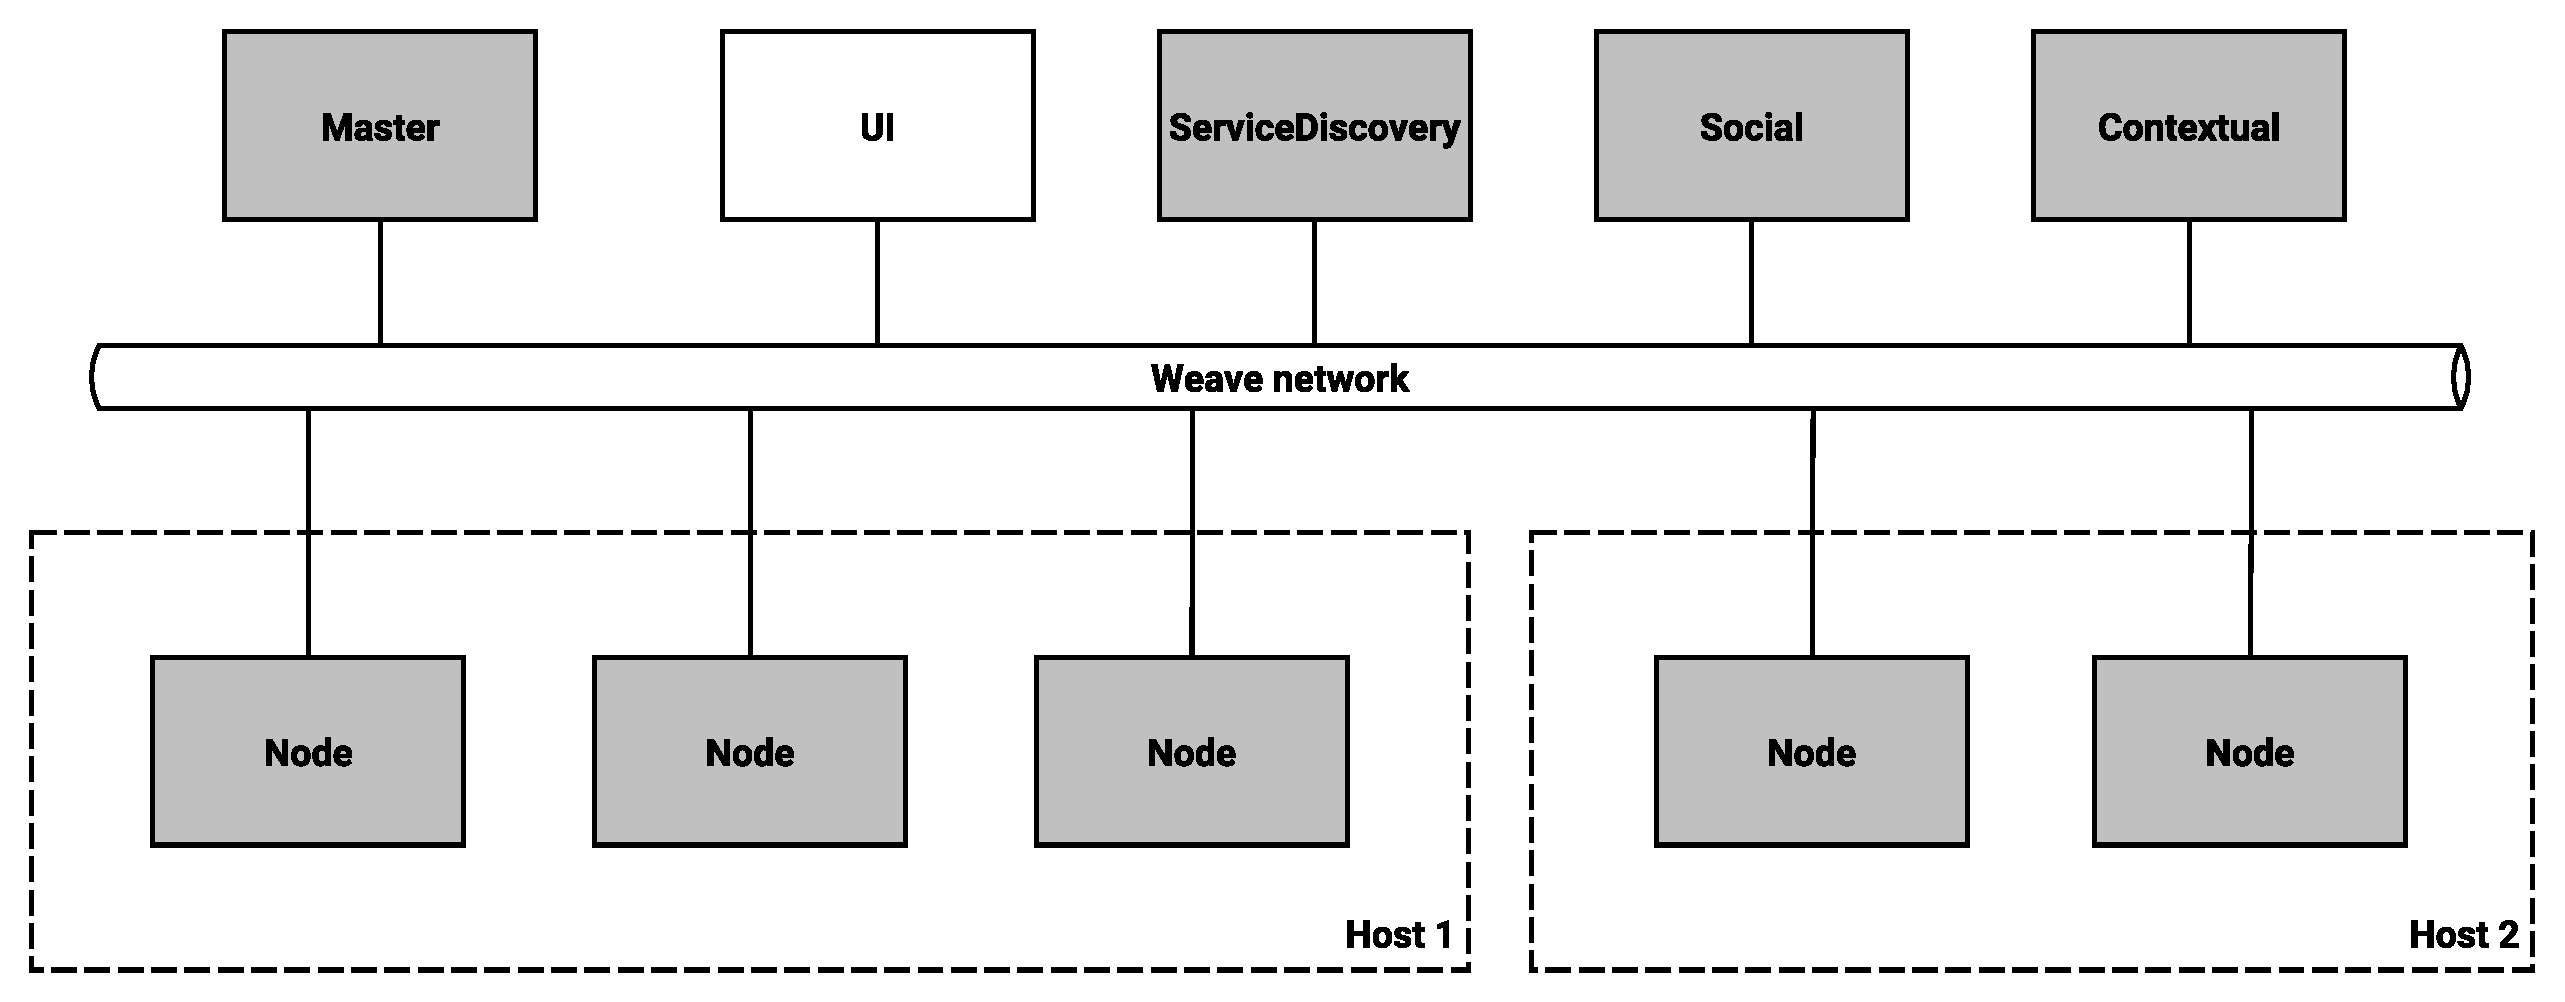
\includegraphics[width=\textwidth]{figures/androfleet}
    \caption{\label{AndroFleet} AndroFleet architecture}
\end{figure*}

The architecture of AndroFleet, presented in the Figure~\ref{AndroFleet}, is composed of 5 elements: Master, Node, ServiceDiscovery, Social, Contextual and UI.
All these elements are packaged and regrouped in a single Docker container.
This container includes an Android emulator that will be run by the Node.

The Master is the main element of the architecture.
It communicates with all other elements of the platform.
For instance, this element is responsible to attribute a scenario to each node container connected.
The Master synchronizes elements of the system.
It allows to control emulation steps with a Command Line Interface and provides information about the progress of the emulation.

The Node element is responsible to launch the Android emulator included in the container and play a GPS scenario.

The ServiceDiscovery element is used for the Wi-Fi Direct simulator.
It allows to the devices to discover themselves.
A Node can request it a list of all its neighbors given its current GPS position.

The Social elements contain information of existing links that exist between emulated users.
The element generates for each running Node its social links.

The Contextual element has the same behaviour as the Social one.
This element generates contextual information for each Node.

The UI is an optional part that can be used to visualize the GPS position of each Android emulator on a map.

A GeoLife parser is included.
It permits to recreate files that are used in our experiment.

\subsection{Evaluation Protocol}

We project to evaluate our approach with our AndroFleet platform.

In the Geo-privacy field, it exists many datasets of real human GPS traces.
One of those is the Microsoft’s GeoLife dataset and is largely used to conduct evaluations.
GeoLife is a GPS trajectory dataset collected from 182 different users in a period of over 3 years. 
This dataset contains a total of 17,621 trajectories.
Because this is the reference dataset, we will process the traces to include it in AndroFleet.

AndroFleet takes a Tick value that allow to configure the time between each location change (if there is one for a user).
We set this Tick value to 5 seconds because in GeoLife, there is about 90\% of data logged that are spaced under 5 seconds.
So each 5 seconds, each Node in AndroFleet will play the next step in its scenario.
This will reproduce the users' movement. 

For the data dissemination testing, we will attribute to each user 5 data and run the emulation.
Because each data has an identifier, it will be possible to study the dissemination of a specific data.

We will add an end-server to AndroFleet to collect data.
We will study the link-ability of the data and see if it will be possible to deduce the producer of those.

%%%% END OK